% TikZ代码:Hash约束引导解空间探索图
% 用于Design章节 - Parameter Space Exploration小节

\documentclass[tikz,border=10pt]{standalone}
\usepackage{tikz}
\usepackage{xcolor}
\definecolor{myred}{HTML}{C00000}
\usetikzlibrary{shapes,arrows,positioning}

\begin{document}

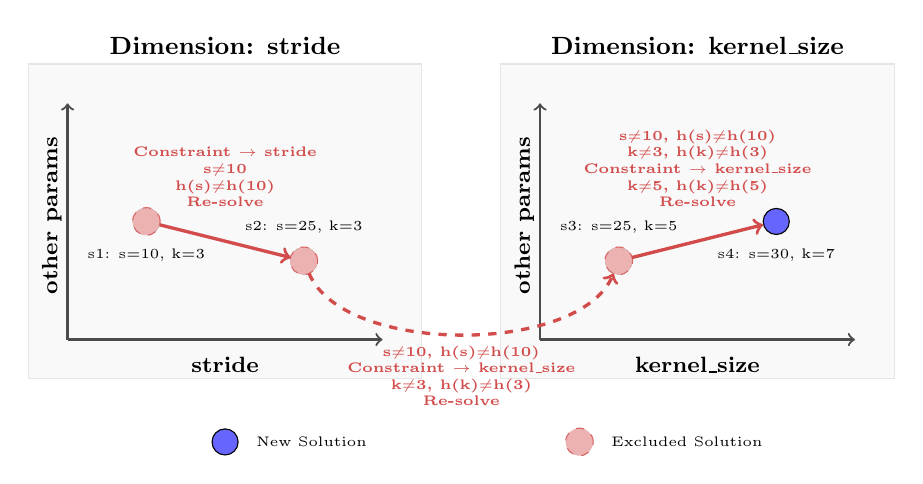
\begin{tikzpicture}[
    scale=1.0,
    dot/.style={circle, fill=blue!60, draw=black, minimum size=0.25cm},
    excluded/.style={circle, fill=myred!30, draw=myred!60, dashed, minimum size=0.35cm},
    label/.style={font=\tiny},
]

% 维度1:stride参数维度
\draw[gray!20, fill=gray!5] (0,0) rectangle (5,4);
\node[above] at (2.5,4) {\small \textbf{Dimension: stride}};

% 维度1的坐标轴
\draw[->, thick, black!70] (0.5,0.5) -- (4.5,0.5);
\node[below=0.1cm, font=\footnotesize\bfseries] at (2.5,0.5) {stride};
\draw[->, thick, black!70] (0.5,0.5) -- (0.5,3.5);
\node[left=0.2cm, font=\footnotesize\bfseries, rotate=90] at (0.5,3.2) {other params};

% 维度2:kernel_size参数维度
\draw[gray!20, fill=gray!5] (6,0) rectangle (11,4);
\node[above] at (8.5,4) {\small \textbf{Dimension: kernel\_size}};

% 维度2的坐标轴
\draw[->, thick, black!70] (6.5,0.5) -- (10.5,0.5);
\node[below=0.1cm, font=\footnotesize\bfseries] at (8.5,0.5) {kernel\_size};
\draw[->, thick, black!70] (6.5,0.5) -- (6.5,3.5);
\node[left=0.2cm, font=\footnotesize\bfseries, rotate=90] at (6.5,3.2) {other params};

% 维度1中的解点
\node[dot] (s1) at (1.5,2) {};
\node[excluded] at (1.5,2) {};
\node[label, below=0.05cm of s1, align=center] {s1: s=10, k=3};

\node[dot] (s2) at (3.5,1.5) {};
\node[excluded] at (3.5,1.5) {};
\node[label, above=0.05cm of s2, align=center] {s2: s=25, k=3};

% 维度2中的解点(显示完整参数组合)
\node[dot] (s3) at (7.5,1.5) {};
\node[excluded] at (7.5,1.5) {};
\node[label, above=0.05cm of s3, align=center] {s3: s=25, k=5};

\node[dot] (s4) at (9.5,2) {};
\node[label, below=0.05cm of s4, align=center] {s4: s=30, k=7};

% 探索路径箭头
% 箭头1:从s1到s2,随机选择stride维度添加约束
\draw[->, myred!70, very thick] (s1) -- node[above=0.3cm, font=\tiny\bfseries, align=center] {Constraint $\rightarrow$ stride \\ s$\neq$10 \\ h(s)$\neq$h(10) \\ Re-solve} (s2);

% 箭头2:从s2到s3,随机选择kernel_size维度添加约束
\draw[->, myred!70, very thick, dashed] (s2) .. controls (4,0.3) and (7,0.3) .. node[below, font=\tiny\bfseries, align=center] { s$\neq$10, h(s)$\neq$h(10) \\ Constraint $\rightarrow$ kernel\_size \\ k$\neq$3, h(k)$\neq$h(3) \\ Re-solve} (s3);

% 箭头3:从s3到s4,随机选择kernel_size维度添加约束
\draw[->, myred!70, very thick] (s3) -- node[above=0.3cm, font=\tiny\bfseries, align=center] { s$\neq$10, h(s)$\neq$h(10) \\ k$\neq$3, h(k)$\neq$h(3) \\ Constraint $\rightarrow$ kernel\_size \\ k$\neq$5, h(k)$\neq$h(5) \\ Re-solve} (s4);

% 图例(在图片下方居中,均匀分布)
% Solution
\node[dot] (leg1_sym) at (2.5,-0.8) {};
\node[label, right=0.1cm of leg1_sym, anchor=west] {New Solution};

% Excluded solution
\node[excluded] (leg2_sym) at (7,-0.8) {};
\node[label, right=0.1cm of leg2_sym, anchor=west] {Excluded Solution};

\end{tikzpicture}

\end{document}
